%%
%% This is file `sample-manuscript.tex',
%% generated with the docstrip utility.
%%
%% The original source files were:
%%
%% samples.dtx  (with options: `all,proceedings,bibtex,manuscript')
%% 
%% IMPORTANT NOTICE:
%% 
%% For the copyright see the source file.
%% 
%% Any modified versions of this file must be renamed
%% with new filenames distinct from sample-manuscript.tex.
%% 
%% For distribution of the original source see the terms
%% for copying and modification in the file samples.dtx.
%% 
%% This generated file may be distributed as long as the
%% original source files, as listed above, are part of the
%% same distribution. (The sources need not necessarily be
%% in the same archive or directory.)
%%
%%
%% Commands for TeXCount
%TC:macro \cite [option:text,text]
%TC:macro \citep [option:text,text]
%TC:macro \citet [option:text,text]
%TC:envir table 0 1
%TC:envir table* 0 1
%TC:envir tabular [ignore] word
%TC:envir displaymath 0 word
%TC:envir math 0 word
%TC:envir comment 0 0
%%
%% The first command in your LaTeX source must be the \documentclass
%% command.
%%
%% For submission and review of your manuscript please change the
%% command to \documentclass[manuscript, screen, review]{acmart}.
%%
%% When submitting camera ready or TAPS, please change the command
%% to \documentclass[sigconf]{acmart} or whichever template is required
%% for your publication.
%%
%%
\documentclass[manuscript,screen,review]{acmart}
%%
%% \BibTeX command to typeset BibTeX logo in the docs
\AtBeginDocument{%
  \providecommand\BibTeX{{%
    Bib\TeX}}}

\usepackage{enumitem}
\usepackage{array}
\usepackage{placeins}
\usepackage{algorithm}
\usepackage{algorithmic}
\usepackage{booktabs} % Required for toprule, midrule, bottomrule
% Prefer vector (PDF) charts when available; fallback to PNG/JPG.
\usepackage{ifthen}
\newcommand{\includebestgraphics}[2][]{%
    % #1 = optional includegraphics options, #2 = base filename without extension
    \IfFileExists{#2.pdf}{%
        \includegraphics[#1]{#2.pdf}%
    }{\IfFileExists{#2.png}{%
        \includegraphics[#1]{#2.png}%
    }{\IfFileExists{#2.jpg}{%
        \includegraphics[#1]{#2.jpg}%
    }{%
        \PackageWarning{includegraphics}{File `#2' not found with .pdf/.png/.jpg extensions}%
    }}}
}
%% Rights management information.  This information is sent to you
%% when you complete the rights form.  These commands have SAMPLE
%% values in them; it is your responsibility as an author to replace
%% the commands and values with those provided to you when you
%% complete the rights form.
\setcopyright{none}
\copyrightyear{2026}
\acmYear{2026}
\acmDOI{XXXXXXX.XXXXXXX}
\acmISBN{978-1-4503-XXXX-X/2018/01}
% \acmISBN{}
%% These commands are for a PROCEEDINGS abstract or paper.
% \acmConference[Conference acronym 'XX]{Make sure to enter the correct
%   conference title from your rights confirmation email}{June 03--05,
%   2018}{Woodstock, NY}
\acmConference[Under Review]{Submitted to ACM Conference}{2026}{Location To Be Decided}


%%
%% Submission ID.
%% Use this when submitting an article to a sponsored event. You'll
%% receive a unique submission ID from the organizers
%% of the event, and this ID should be used as the parameter to this command.
%%\acmSubmissionID{123-A56-BU3}

%%
%% For managing citations, it is recommended to use bibliography
%% files in BibTeX format.
%%
%% You can then either use BibTeX with the ACM-Reference-Format style,
%% or BibLaTeX with the acmnumeric or acmauthoryear sytles, that include
%% support for advanced citation of software artefact from the
%% biblatex-software package, also separately available on CTAN.
%%
%% Look at the sample-*-biblatex.tex files for templates showcasing
%% the biblatex styles.
%%

%%
%% The majority of ACM publications use numbered citations and
%% references.  The command \citestyle{authoryear} switches to the
%% "author year" style.
%%
%% If you are preparing content for an event
%% sponsored by ACM SIGGRAPH, you must use the "author year" style of
%% citations and references.
%% Uncommenting
%% the next command will enable that style.
%%\citestyle{acmauthoryear}


%%
%% end of the preamble, start of the body of the document source.
\begin{document}

%%
%% The "title" command has an optional parameter,
%% allowing the author to define a "short title" to be used in page headers.
\title[]{Guiding End-Users towards Software Reuse: An Evaluation of Automated Assistance in Block-Based Programming for Chemistry Laboratory Automation}

%%
%% The "author" command and its associated commands are used to define
%% the authors and their affiliations.
%% Of note is the shared affiliation of the first two authors, and the
%% "authornote" and "authornotemark" commands
%% used to denote shared contribution to the research.
\author{Anne-Marie Rommerdahl}
\affiliation{%
 \institution{SDU}
 \city{Odense}
 \country{Denmark}}
\email{anrom25@student.sdu.dk}

\author{Jeremy Alexander Ramírez Galeotti}
\affiliation{%
 \institution{SDU}
 \city{Odense}
 \country{Denmark}}
\email{jeram25@student.sdu.dk}

\author{Dimitrios Dafnis}
\affiliation{%
 \institution{SDU}
 \city{Odense}
 \country{Denmark}}
\email{didaf25@student.sdu.dk}

\author{Nasifa Akter}
\affiliation{%
 \institution{SDU}
 \city{Copenhagen}
 \country{Denmark}}
\email{naakt23@student.sdu.dk}

\author{Mohammad Hosein Kardouni}
\affiliation{%
 \institution{SDU}
 \city{Odense}
 \country{Denmark}}
\email{mokar25@student.sdu.dk}



%%
%% By default, the full list of authors will be used in the page
%% headers. Often, this list is too long, and will overlap
%% other information printed in the page headers. This command allows
%% the author to define a more concise list
%% of authors' names for this purpose.
\renewcommand{\shortauthors}{Anne-Marie Rommerdahl, Jeremy Galeotti, Dimitrios Dafnis, Nasifa Akter, Mohammad Kardouni}

%%
%% The abstract is a short summary of the work to be presented in the
%% article.
\settopmatter{printacmref=true, printccs=true, printfolios=true} % Remove ACM Reference Format and copyright info
% \renewcommand\footnotetextcopyrightpermission[1]{} % Remove copyright footer
\begin{CCSXML}
<ccs2012>
   <concept>
       <concept_id>10011007.10011074.10011092.10011096</concept_id>
       <concept_desc>Software and its engineering~Reusability</concept_desc>
       <concept_significance>500</concept_significance>
       </concept>
 </ccs2012>
\end{CCSXML}

\ccsdesc[500]{Software and its engineering~Reusability}

\begin{abstract}


\noindent\textbf{\textit{Abstract}—End-users who program collaborative robots for laboratory automation often create repetitive code because they struggle to recognize opportunities for reuse. While block-based programming environments provide accessible interfaces, 
they do not actively guide end-users toward creating reusable components. This study investigates whether automated guidance can help end-users recognize and apply code reuse practices. We developed the Reuse Assistant, 
a feature that automatically detects duplicate code sequences within the OpenRoberta environment and guides users to create reusable custom blocks through visual highlighting and one-click refactoring. Through a 
within-subjects study with 18 participants from the chemistry domain, we evaluated the feature's impact on performance, usability, and perceived workload.
Automated guidance increased reuse adoption from 0\% in the standard OpenRoberta version to 100\% when using the Reuse Assistant. The feature achieved high usability scores (SUS mean: 84.03) and imposed minimal 
cognitive burden (NASA-TLX mean score: 1.92). The significant carryover effect revealed that prior manual experience helps users appreciate automation benefits.
This dramatic shift in adoption suggests that end-users are capable of using advanced features if the system actively guides them.}
%However, the order effect suggests that some manual experience is necessary to fully benefit from automation. Participants who struggled with manual coding first developed a mental model that allowed them to better appreciate and efficiently use the automated assistance.}
%Last part is basically the part of implications for practice that thiago told us to remove, so lets cut it out as well





\end{abstract}

\maketitle
%%
%% This command processes the author and affiliation and title
%% information and builds the first part of the formatted document.

%%
%% The code below should be generated by the tool at
%% https://dl.acm.org/ccs.cfm
%% Please copy and paste the code instead of the example below.
%%


%%
%% Keywords. The author(s) should pick words that accurately describe
%% the work being presented. Separate the keywords with commas.
\keywords{end-user development, block-based programming, code reuse, automated guidance, laboratory automation, collaborative robots, usability, attention investment model, learning barriers}


\section{Introduction}

Software reuse is a fundamental practice in software engineering, enabling developers to build on existing solutions rather than 
writing code from scratch. However, end-users who program collaborative robots (cobots) for laboratory automation often lack the 
knowledge to recognize and apply reuse opportunities. This problem is particularly acute in domains like chemistry, where scientists 
need to automate repetitive experimental procedures but have limited programming expertise.

Block-based programming environments such as OpenRoberta Lab provide accessible interfaces for programming robots, but they do not 
actively guide users toward creating reusable components. As a result, end-users frequently produce long, repetitive programs that are 
difficult to maintain and modify. When experimental protocols change, users must manually update code in multiple locations, increasing 
the risk of errors and discouraging adoption of automation features.

This study addresses the question: Can automated guidance help end-users recognize and apply code reuse in block-based programming? 
We developed the Reuse Assistant, a feature that automatically detects duplicate code sequences and guides users to create reusable custom 
blocks through visual highlighting and one-click refactoring. Through a within-subjects study with 18 participants from the chemistry domain, 
we evaluated whether proactive automated assistance can overcome the barriers that prevent end-users from adopting reuse practices.

Our investigation examined four research questions: 
\begin{enumerate}[nosep, label=\textbf{\arabic*)}]
    \item How does the Reuse Assistant affect the end-users' performance?
    \item To what extent does the reuse assistant facilitate reusability?
    \item How do the end-users assess the reuse assistant in terms of usability?
    \item How do the end-users assess the perceived workload when operating the Reuse Assistant?
\end{enumerate}
    
The results showed that automated guidance increased reuse adoption from 0\% to 100\%, achieved high usability scores (SUS mean: 84.03), and imposed minimal cognitive burden (NASA-TLX mean score: 2).

The contributions of this work are both theoretical and practical. We extend the Attention Investment Model \cite{BlackwellAttentionInvestment} 
and Learning Barriers Framework \cite{KoLearningBarriers} by demonstrating that proactive assistance transforms feature adoption from a high-cost investment to a low-cost opportunistic choice, 
effectively reducing the selection barrier. 
%However, we also identify a critical "order effect," suggesting that manual experience is a prerequisite for maximizing the efficiency of automated tools. 
%From a practical perspective, our results show that while simple design principles (visual highlighting, one-click acceptance) achieve high usability, the most effective adoption occurs when automation is introduced after users have developed a mental model of the manual process.
% Also outcommenting this, as this is also about the implications for practice that thiago wanted removed



\section{Background and Related Work}
\label{sec:background_relatedWork}
%% ---- Background ----
%% 1 Background abt. reuse. What is it, and why is it important? (anne)
%% 2 What is the current state of 'reuse' for low-code? Anne paragraph (anne)
%% 3 In what ways have different low-code tools tackled 'reuse'? We look at different low-code tools, not just block-based ones. What are the strengths and weaknesses of their approach to reuse? MAKE SURE TO MENTION TOOLS BY NAME! (dimitris)
%% 4 Now we look at block-based tools for robots (for example, scratch, VEXcode GO, OpenRoberta). How do they tackle reuse? (jeremy + Mohamad)
%% 5 Based on the identified weaknesses in current practices for reuse, we propose our own idea (explain how it's gonna work) (Nasifa)

%% ----Re-done intro----
Software reuse is the practice of reusing previously written code, rather than writing new code from scratch. It is such an important part of software engineering, that one of the ways to measure the quality of software is by its 'Reusability'\cite{SoftwareArchitectureInPractice}, i.e. the degree to which the application or its components can be reused. 
There are multiple benefits to practicing reuse in software engineering. One developer could save time by using another developer's reusable component, rather than coding their own. The developer avoids both the work of writing the syntax and designing the logic of the component. The developer can also design their own reusable components, keeping all the logic in one place, making both testing and maintenance easier to perform. However, despite reuse being an important practice in software engineering, there is still a limited focus on this practice when it comes to low-code development platforms (LCDP).

%%--from here: what reuse is there for low-code? What research? IN GENERAL
%%-- Then, what tools? examples of how tools tackle reuse
%%-- Then, what tools for blocks and robots? How do they tackle reuse? What are their strengths/weaknesses/limitations? MAKE SURE TO MENTION BY NAME!!
%%-- Show the tool we'll be working on (what does it do for reuse, and weaknesses).
%%-- Based on all that, what is our idea? What gap is it, we're addressing and how?
%% ---------------------
A study by Bock and Frank (2021) studied several low-code platforms (LCPs), in order to identify characteristic features of LCPs. The identified features were presented according to how frequently they occured, with domain-specific reference artifacts being categorized as 'rare'. Most studied systems offered catalogs of "reusable functions or examples of predefined processes", but they were found to be generic, or have a limited scope\cite{LowCodePlatform}. This lack of focus on promoting reuse may impact the so-called 'Citizen Developers', who have little or no coding knowledge, and whom may then miss out on the benefits of reuse. Lin and Weintrop (2021) noted that most existing research on block-based programming focuses on supporting the transition to text-based languages rather than exploring how features within BBP environments, such as abstraction or reuse, can enhance learning outcomes\cite{Lin2021Landscape}.

There have been proposed some ideas on how to promote reuse for LCPs, such as the templating language OSTRICH, developed for the model-driven low-code platform OutSystems\cite{OSTRICH}. OSTRICH is designed to assist the end-user in making use of OutSystems' available templates, by abstracting and parameterizing the templates. However, OSTRICH only supports the top nine most used production-ready screen templates, and does not allow the end-user to create and save their own templates, or re-apply a template which they have customized. Another approach focused on enabling the reuse of models, by providing recommendations to the end-user, based on the models stored in a graph acting as a repository. While the graph allows end-users to reuse their own models, there is no mention of guiding the user towards reusing their own models.

%Low code platform tools that focus on reuse
%[x does this, y does that, but a common trend seen in all of them is the almost nonexistent guidance towards using these features. If a user doesnt know/care about reuse, that mentality is never challenged.]
Several popular low-code development platforms (LCDPs) provide different kinds of support for reuse. Webflow\cite{webflow}, a LCDP for responsive websites, offers the ability to create reusable components and UI kits, which can be reused across multiple pages and projects. 
Mendix\cite{mendix} and OutSystems offer even more functionality to support reuse, offering several ways to end-users to share their code with each other, and offering pre-made components. Both of these platforms also utilize AI to enhance reuse. Outsystems provides AI suggestions to spot and create reusable pieces, while Mendix uses AI to suggest the best solutions and components for specific tasks. 
However, well-known pitfalls of AI are its tendency to generate non-deterministic outputs, and hallucinations. While an experienced programmer can critically analyze the output of the AI, the common end-user lacks that ability. %However, for both of these platforms, the AI suggestions provided are not always accurate to successfully guide the end-user to create custom reusable components.\\
In order to analyze how block-based robotics environments address reuse, 4 representative platforms were compared: mBlock, MakeCode, SPIKE LEGO, VEXcode GO and Open Roberta. The comparison focused on three main dimensions of reuse: structural reuse (through user-defined blocks or functions), social reuse (through sharing or remixing existing projects), and interoperable reuse (through import/export capabilities).
\begin{table}[H]
  \small   
  \caption{Block Based Robotics Environments Reuse Support}
  \label{tab:reuse_support}
  \begin{tabular}{lcccc}
    \toprule
    Platform & Structural Reuse & Social Reuse & Interoperable Reuse & Reuse Support \\
    \midrule
    VEXcode GO    & X & X &  & Medium \\
    mBlock        & X & X & X & Medium \\
    MakeCode      & X & X & X & Medium \\
    Spike Lego    & X &  & X & Low \\
    Open Roberta  &  & X &  & Low \\
    \bottomrule
  \end{tabular}
\end{table}
In this context, “reuse support” represents a scale that measures how effectively each platform facilitates reuse-related features. High reuse support indicates that users can easily create, share, and adapt existing components or projects. Medium reuse support suggests that some reuse mechanisms are available but limited in scope or flexibility. Low reuse support implies that the platform provides only minimal or restricted features to promote reuse.

As shown in Table \ref{tab:reuse_support}, although these platforms include reusability features, they are quite limited, as none of them provide users with clear guidance on how to use these tools effectively, which restricts their ability to fully leverage them.\\\\
A study by Techapalokul and Tilevich (2019) suggests that supporting mechanisms for reusing smaller, modular pieces of code can enhance programmer productivity, creativity and learning outcomes. 
Adler et al. (2021) introduced a search-based refactoring approach to improve the readability of Scratch programs by automatically applying small code transformations, such as simplifying control structures and splitting long scripts\cite{Adler2021Improving}. Their findings demonstrated that automated refactoring can significantly enhance code quality and readability for novice programmers. 

Building upon all these concepts and ideas, our project introduces a guided Reuse Assistant feature within the OpenRoberta Lab environment. The feature is designed to help users identify and apply reuse more easily while creating their robot programs. Focused on guiding users toward creating reusable custom blocks to promote modularity and abstraction, the feature automatically scans a user's block-based program to detect repeated code segments in the workspace. The system visually highlights the found duplicates, drawing the user’s attention to patterns that can be reused. The feature also offers the functionality to create the custom block for the end-user, by identifying the small differences between the repeated parts (such as numbers, variables, or parameters) and turning these differences into inputs for the new block. The feature automatically replaces all relevant duplicate sequences with the new custom block.

By combining ideas from procedural abstraction (organizing code into meaningful, reusable parts) and automated refactoring (improving code through intelligent transformations), our feature aims to make block-based programming more structured and efficient.
It encourages users to build programs that are modular and easier to maintain, helps reduce unnecessary repetition, and supports learning by making the concept of reuse clear and hands-on.
%In summary, our work bridges the gap between existing theoretical approaches to software reuse and their real-world application in block-based programming environments. Through this guided and semi-automated approach, we aim to make reuse visible, understandable, and practical for end-users working in Open Roberta.

\section{Study Design}
\label{sec:study_design}
Following the Design Science methodology \cite{Wieringa2014}, the study is structured into three main phases: 
problem investigation to define goals, treatment design to specify the artifact requirements, and treatment validation to 
assess the artifact's performance in a controlled environment.

\subsection{Problem Investigation}
\label{subsec:prob_investigation}

\subsubsection{Problem Context and Motivation}
End-user development (EUD) for collaborative robots (cobots) presents unique challenges, particularly for users without 
formal programming training. In domains such as chemistry, educational robotics, and industrial settings, 
end-users need to program 
robots to perform specific tasks but often lack the software engineering knowledge to write maintainable, well-structured 
code.
In the domain of Chemistry, one of the most relevant and important tasks is performing experiments in labs. %in order to test a hypothesis, or to aid in the understanding of how chemicals react. 
Robots can be used in chemistry labs to automate 
experiments with great effect, as many experiments involve steps that are repetitive, and susceptible to human error, 
such as a step being overlooked, instructions being misread, etc. Automation of menial tasks will leave the chemists with 
more time for other work, with the added bonus of not having to handle dangerous chemicals.\\
One critical challenge in EUD is code reuse. Users frequently create repetitive code as they struggle to recognize 
duplicate patterns, lack knowledge about abstraction mechanisms, or find existing tools too complex to use effectively. 
This problem manifests in several ways: programs become unnecessarily long and difficult to maintain and small changes 
require modifications in multiple locations, increasing the risk of errors. So, while the use of robots in chemistry lab 
work offer great benefits, the challenge of automating the repetitive work may turn chemists away from using robots.

\subsubsection{Stakeholder Analysis}
Chemists and lab technicians who use cobots for repetitive tasks such as sample preparation, mixing, quality control procedures, etc. 
They possess deep domain expertise in chemistry but limited programming knowledge, often creating long, repetitive programs that become difficult to maintain when adapting experimental protocols. 
Their primary need is to quickly create and modify robot programs without becoming programming experts.


\subsection{Treatment Design}
\label{subsec:treatment_design}
To address the problem of code reuse in EUD for cobots, we have derived a set of requirements designed to contribute to 
the chemist's goal of creating maintainable and reusable robot programs.
Functionally, the artifact must be capable of automatically detecting duplicate or similar block sequences and visually 
highlighting these duplications within the user's workspace.
These requirements are necessary to help the end-user recognize opportunities for reuse, that would otherwise go 
unnoticed. Once detected, the system must offer to create reusable custom blocks, allowing the user to accept or 
reject these suggestions.
These signals are important, as they give the end-user control over the reuse process, allowing them to decide when and 
how to apply reuse in their programs.
Regarding non-functional requirements, the artifact must seamlessly integrate with the existing Open Roberta Lab 
environment to ensure a smooth user experience.
The interface should be intuitive for end-users, minimizing the learning curve and making it easy to understand and use 
the reuse features. Additionally, the artifact should not interfere with the existing workflow, allowing users to continue 
their programming tasks without disruption. %Finally, clear visual feedback during the detection process is essential to help users understand what the system is doing and how to respond to its suggestions.
% this is already mentioned further up. 
To satisfy the requirements above, we designed the Reuse Assistant (source code available at: \url{https://github.com/jim-daf/end_user_deploy}) as a feature for the Open Roberta Lab. 


\subsubsection{Architecture}

The system enables the execution of block-based programs on a simulated cobot through a three-tier architecture, as illustrated in figure \ref{fig:architecture}. The workflow consists of the following stages:

\begin{enumerate}
    \item \textbf{Client Side (Open Roberta):} The user interacts with the Open Roberta UI to assemble block sequences. The Reuse Assistant operates at this layer, analyzing blocks in real-time. Upon execution, the client generates specific data structures ("Generated Headers") representing the program logic.
    \item \textbf{Backend (Flask Server):} The client transmits these headers via HTTP GET requests to a Flask-based API Endpoint. A "Translator" component processes the data, mapping the abstract block definitions to concrete Python methods compatible with the robot's control logic. %Its GET, not POST
    \item \textbf{Simulation (Mujoco):} The mapped methods trigger the execution of commands within the Mujoco Simulator, which renders the physical behavior of the cobot in the virtual environment.
\end{enumerate}


% FIX FIGURE - GET, remove 'translation'
% Zoomed version of the architecture figure on its own page
\begin{figure}[ht] 
    \centering
    % width=\textwidth ensures it fills the page width
    % keepaspectratio ensures it doesn't get distorted
    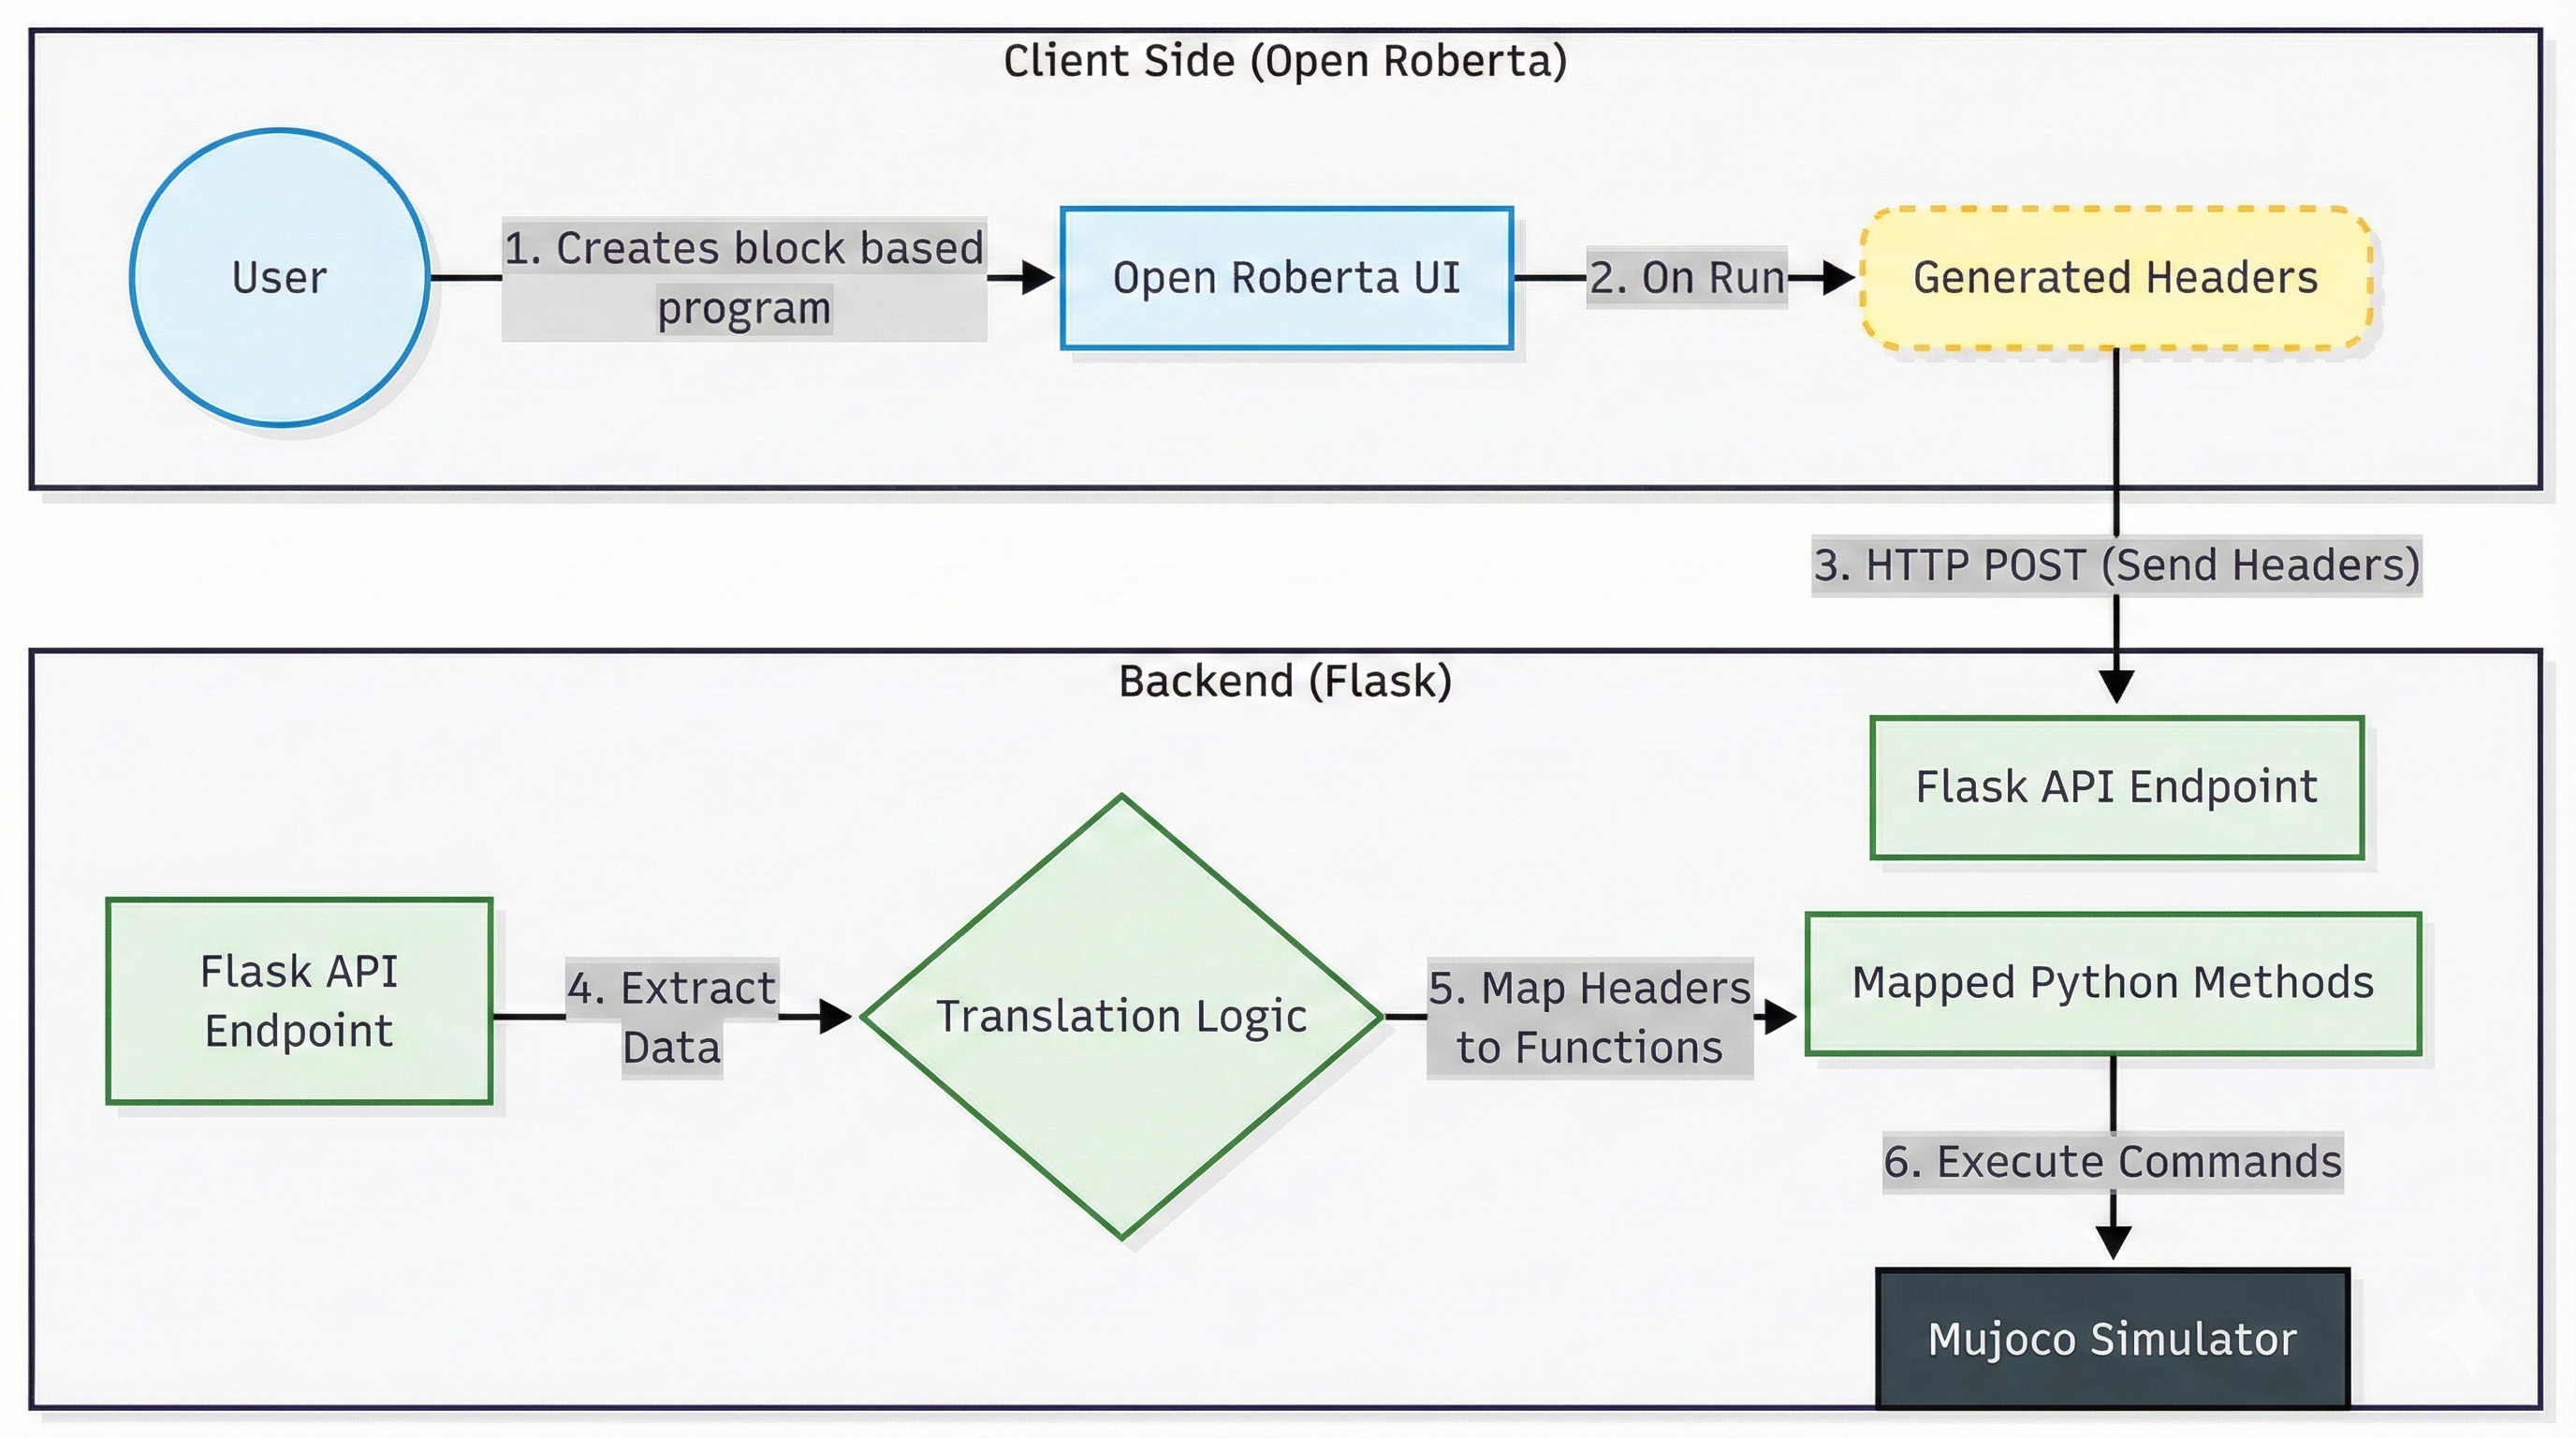
\includegraphics[width=0.81\textwidth, keepaspectratio]{images/ArchitectureH2.png}
    \caption{System architecture: Data flow from Client Side to Simulator}
    \label{fig:architecture}
\end{figure}

\FloatBarrier

\subsubsection{Detection Algorithm}
%The approach is intentionally simple so it is easy to read and to implement in a real block editor. 
% this sentence is irrelevant. Also, whats a 'real block editor'? 
The algorithm follows three main steps:
\begin{itemize}[nosep]
    \item \textbf{Linearization:} First, the algorithm linearizes the block workspace into a sequential list of blocks. 
    \item \textbf{Identify sequences:} It iterates through this list to identify all possible sequences of blocks that meet a minimum unique block type length requirement (three blocks). % that can be repeated more than once.
    % Every block sequence can be repeated more than once? So unecessary?
    \item \textbf{Sequences Matching:} If the same sequence of block types is found more than once, it will be added to the ReusableComponentCandidates list, which will be sorted by longest and most recent duplicated sequences. In the end the highest priority candidate gets returned.
\end{itemize}
The pseudocode is illustrated in Algorithm~\ref{alg:detection_refined}.
%The pseudocode which is illustrated in Algorithm~\ref{alg:detection_refined} is short, explicit, and uses straightforward data structures (lists).
\begin{algorithm}[ht]
\caption{Illustrates the core logic for identifying duplicate block sequences in the user's workspace.}
\label{alg:detection_refined}
\begin{algorithmic}[1]
\REQUIRE Workspace, StartBlock \quad // user's block workspace
\REQUIRE MinimumSequenceLength = 3, MinimumDifferentBlockTypesInSequence = 3, MaxSequenceLength = 10 \quad
\ENSURE ReusableComponentCandidates \quad // list of repeated block sequences to return
\STATE Chain $=$ \textbf{buildLinearChain}(StartBlock) 
\STATE Sequences $=$ List$\langle$sequence$\rangle$ 

\FOR{startIndex = 0 \TO length(Chain) - 1} 
    \FOR{$sequenceLength = 1$ \TO $MaxSequenceLength$ }
        \STATE sequence $=$ Chain[startIndex \,..\, startIndex + sequenceLength - 1] 
        \STATE numberOfBlockTypesInSequence = getNumberOfDistinctBlockTypes(sequence)
        \IF{sequenceLength >= MinimumSequenceLength \textbf{ and } numberOfBlockTypesInSequence >= MinimumDifferentBlockTypesInSequence}
            \STATE Sequences.append(sequence) // record sequence occurrence
        \ENDIF
    \ENDFOR
\ENDFOR

\STATE ReusableComponentCandidates $= \{\text{Sequences} \mid occurrence \ge 2 \}$ 
\STATE sort ReusableComponentCandidates by (longest sequence length and most recent occurrence) 
\RETURN ReusableComponentCandidates[0] // Return highest priority candidate
\end{algorithmic}
\end{algorithm}

\vspace{-5mm}
\subsubsection{User Interface and Interaction}
The user interface is designed to be intuitive and as non-disruptive as possible. When the detection algorithm identifies a candidate, the system visually highlights the relevant blocks on the canvas as shown in Figure \ref{fig:ui_interaction_highlight}. A toast notification appears, prompting the user to confirm the refactoring. The workspace is blocked until the user gives an answer (ideally, this notification should be non-blocking, and we consider this a limitation of the feature). If the user confirms, the system automatically generates the custom block definition in a dedicated workspace area and updates the main workspace, replacing the redundant code with concise function calls as shown in Figure \ref{fig:ui_interaction_refactor}.
%If confirmed, the system automatically generates the custom block definition in a dedicated workspace area (handling visibility via \texttt{revealDefinitionWorkspacePane}) and updates the main workspace, replacing the redundant code with concise function calls as shown in Figure \ref{fig:ui_interaction_refactor}. 
% The reader doesn't know what revealDefinitionWorkspacePane is. We shouldn't mention parts of the code that we don't explicitly show in the report
This process abstracts the complexity of manual function creation, guiding the user toward modular design practices. 
After the user presses the run simulation button, the robot simulator of mujoco opens up and executes the commands provided by the user inside the Open Roberta workspace. This is illustrated in Figure \ref{fig:mujoco_simulator}.

% --- START: Split UI figures ---

\vspace{-1mm}
\begin{figure}[h]
    \centering
    % Prefer vector PDF when available, fallback to PNG/JPG
    \includebestgraphics[width=0.85\linewidth]{images/updatedHighlight}
    \Description{A screenshot of the Open Roberta environment. Two identical sequences of blocks are highlighted. A pop-up message in the bottom right asks the user if they want to create a reusable block.}
    \caption{Reuse Assistant workflow: detection - the interface highlights detected duplicate blocks by changing their color to green.}
    \label{fig:ui_interaction_highlight}
\end{figure}
\begin{figure}[h]
    \centering
    % Prefer vector PDF when available, fallback to PNG/JPG
    \includebestgraphics[width=0.85\linewidth]{images/custom_component}
    \Description{Screenshot showing the code after refactoring. The main program is now much shorter. A side panel shows the definition of the new custom block with parameters for coordinates.}
    \caption{Reuse Assistant workflow: refactoring - the automated refactoring result, showing the new custom block definition and the simplified main program.}
    \label{fig:ui_interaction_refactor}
\end{figure}
\FloatBarrier

\begin{figure}[h]
    \centering
    % Prefer vector PDF when available, fallback to PNG/JPG
    \includebestgraphics[width=0.85\linewidth]{images/mujoco}
    \Description{Screenshot showing the code after refactoring. The main program is now much shorter. A side panel shows the definition of the new custom block with parameters for coordinates.}
    \caption{Mujoco robot simulator executing the commands from Open Roberta.}
    \label{fig:mujoco_simulator}
\end{figure}

% Treatment validation needs to be split into subsections "data gathering and analysis" How we gather the data and how we analyze them
%"Task execution" We need to explain what exactly will be the task
\subsection{Treatment Validation}
\label{subsec:treatment_validation}
% We only collect quantitative data, so its not mixed-method
The treatment validation for this study adopts a quantitative evaluation approach to assess the effectiveness of the proposed features for guiding users in creating custom reusable components (blocks) within the Open Roberta environment. 

\subsubsection{Participant Recruitment}
A total of 18 participants were selected with similar level of expertise in block-based programming. 
Participants were recruited from a diverse pool of individuals affiliated with the University of Southern Denmark and the broader chemistry community. 
This group of participants includes chemistry teachers, professional chemical engineers, and students currently enrolled in chemistry-intensive curricula. 
To ensure relevant practical expertise, the selection specifically targets those who frequently engage in laboratory environments. 
The experimental sessions were conducted across a range of environments to accommodate participant availability. 
Physical sessions took place within the chemistry laboratories at the University of Southern Denmark (SDU) as well as a private residential setting. 
For remote participants, sessions were administered virtually using Discord for communication and AnyDesk for remote desktop control.

% \paragraph{Ethical Considerations and Sampling}
% Prior to the commencement of the study, all participants are required to sign a consent form acknowledging their voluntary participation and granting permission for screen recording and data usage. ----------------------------------------------------------------------
\subsubsection{Task Execution}
The participants were initially given a short introduction to the Open Roberta UI, as well as the mujoco robot simulator. 
They then performed one task which is described by a set of pre-defined steps. This task has been specifically designed to promote the reusability aspect. The task is focused on the domain of chemistry, as it is modelled after a real lab experiment performed by chemistry students at SDU. 

The participants were instructed to program the robot to execute the following sequence of operations:

\begin{enumerate}
    \item Move the robot arm above mix cylinder
    \item Mix the chemistry ingredients
    \item Move the robot arm above the analysis pad
    \item Analyze the sample
    \item If the solution is analyzed (use if statement) then show a response message in the laptop’s screen 
    \item Place the following three objects into their corresponding slots in the chemistry equipment toolbox:
    \begin{itemize}
        \item Methanol cylinder
        \item Chloroform syringe
        \item Toluene syringe
    \end{itemize}
    \item Important notes for the participants:
    \begin{itemize}
        \item \textit{After placing an object to its slot in the toolbox \textbf{wait 2 seconds} before you move to pick a new one.}
        \item \textit{After placing the \textbf{chloroform syringe} to its slot, \textbf{move the robot arm up by 10 cm} before you move to pick the next chemistry object }
        \item \textit{Click the \textbf{play} button on the bottom right corner to start the simulation}
        \item \textit{Click the \textbf{reset} button on the bottom right corner to reset the scene of the robot simulator}
    \end{itemize}
\end{enumerate}

The most optimal solution as defined by the researchers is illustrated in Figure \ref{fig:optimal_solution}.
 \begin{figure}[h]
     \centering
     \includegraphics[width=0.75\textwidth]{images/most optimal solution.png}
     \caption{The optimal solution implemented in OpenRoberta, utilizing a custom block for the object placement sequence.}
     \Description{Block-based program showing the optimal solution with a custom reusable block for placing chemistry objects into toolbox slots.}
     \label{fig:optimal_solution}
 \end{figure}
Instead of creating a long linear sequence of blocks, the most optimal solution utilizes a Custom Reusable Component to handle the repetitive action of placing an object in its corresponding slot inside the equipment toolbox. 
This approach not only reduces redundancy but also enhances code maintainability and readability, aligning with best practices in software development.

%To evaluate the impact of the Reuse Assistant on end-user performance, we measured task completion times for all participants using either version (enhanced or original) of Open Roberta.
% both conditions (Enhanced and Original versions of OpenRoberta). 
%The study employed a within-subjects design where participants were divided into two groups: 
%Group A used the enhanced version of Open Roberta first, while group B started with the Original version. This design allowed us to assess not only the feature's effectiveness but also the potential order effect arising from the learning curve between the two conditions.

All the participants will perform the task using both the enhanced version of Open Roberta, which includes the Reuse Assistant, and the original one which does not. 
The study employs a within-subjects design, where all participants are divided into two groups. Half of the participants (Group A) will first perform the task using the enhanced version, then the original version. The other participants (Group B) will do the opposite order.
Participants’ interactions with the platform will be observed throughout the task.
Guidance will be provided from the researchers to the participants throughout the task.

% -------------------------------------------------------------------------------------------------------------------------------------------------------------------
\subsubsection{Data Gathering and Analysis}
% We dont do qualitative anymore. All results are numerical in nature, so only quantitative
%Data collection focuses on both quantitative performance and qualitative feedback from participants:
The data collection focused on numerical measurements of performance and participant feedback:
\begin{enumerate}
    \item \textbf{Task Completion Time:} Measured in seconds for both versions of Open Roberta (enhanced and original) to evaluate efficiency gains. 
    Statistical analysis employed paired t-tests to assess within-group improvements and a Welch’s t-test to compare improvement scores between groups, specifically isolating the impact of the order effect arising from the sequence of conditions.
    \item \textbf{Reuse adoption:} Evaluated by tracking the voluntary implementation of reusable custom blocks during the task. It was measured how many participants let the Reuse Assistant create custom blocks for them. %This primarily measured adoption rates (pass/fail of reuse implementation). 
    \item \textbf{Usability Assessment:} Evaluated using the System Usability Scale (SUS) questionnaire to measure participants' perceived usability of the Reuse Assistant feature. The SUS yields a single number representing a composite measure of the overall usability of the system, with scores ranging from 0 to 100.
    \item \textbf{Workload Assessment:} Measured using the NASA post-task Workload questionnaire (NASA-TLX) to assess the cognitive demands imposed by the Reuse Assistant across six dimensions (mental demand, physical demand, temporal demand, performance, effort, and frustration).
\end{enumerate}

This comprehensive evaluation provided a detailed understanding of how useful and effective the Reuse Assistant feature is to the 
end-users.
%-------------------------------------------------------------------------------------------------------------------------------------------------------------------
\section{Results}
\subsection{Research Question 1: How does the Reuse Assistant affect the end-users' performance? }
To evaluate the impact of the Reuse Assistant on end-user performance, we measured task completion times for all participants using either version (enhanced or original) of Open Roberta.
% both conditions (Enhanced and Original versions of OpenRoberta). 
%The study employed a within-subjects design where participants were divided into two groups: 
%Group A used the enhanced version of Open Roberta first, while group B started with the Original version. This design allowed us to assess not only the feature's effectiveness but also the potential order effect arising from the learning curve between the two conditions.
% In this section, we focus only on the results. Everything about HOW we gathered the results should be explained in 'Treatment Validation'

Tables \ref{tab:group_a_times} and \ref{tab:group_b_times} present the individual completion times for all participants using either version of Open Roberta. %across both conditions (with and without using the Reuse Assistant). 
The data reveals substantial variability in performance outcomes depending on the order in which the participants performed the tasks, 
with Group B participants showing consistent improvements when moving from the original Open Roberta version to the enhanced, while 
Group A participants exhibited the opposite pattern.

\begin{table}[h]
\centering
\setlength{\tabcolsep}{8pt}
\renewcommand{\arraystretch}{1.3}
\begin{tabular}{|l|r|r|r|}
\hline
\textbf{Participant ID} & \textbf{Performance with Reuse Assistant} & \textbf{Performance without Reuse Assistant} & \textbf{Difference} \\
\hline
P01 & 481 seconds & 331 seconds & 150 seconds \\
\hline
P03 & 515 seconds & 320 seconds & 195 seconds \\
\hline
P06 & 733 seconds & 314 seconds & 419 seconds \\
\hline
P07 & 437 seconds & 296 seconds & 141 seconds \\
\hline
P09 & 453 seconds & 348 seconds & 105 seconds \\
\hline
P11 & 735 seconds & 364 seconds & 371 seconds \\
\hline
P13 & 610 seconds & 407 seconds & 203 seconds \\
\hline
P15 & 410 seconds & 540 seconds & -130 seconds \\
\hline
P17 & 560 seconds & 440 seconds & 120 seconds \\
\hline
\end{tabular}
\caption{Task Completion Times of group A}
\label{tab:group_a_times}
\end{table}

\begin{table}[h]
\centering
\setlength{\tabcolsep}{8pt}
\renewcommand{\arraystretch}{1.3}
\begin{tabular}{|l|r|r|r|}
\hline
\textbf{Participant ID} & \textbf{Performance with Reuse Assistant} & \textbf{Performance without Reuse Assistant} & \textbf{Difference} \\
\hline
P02 & 411 seconds & 477 seconds & -66 seconds \\
\hline
P04 & 189 seconds & 435 seconds & -246 seconds \\
\hline
P05 & 200 seconds & 367 seconds & -167 seconds \\
\hline
P08 & 266 seconds & 485 seconds & -219 seconds \\
\hline
P10 & 259 seconds & 506 seconds & -247 seconds \\
\hline
P12 & 450 seconds & 720 seconds & -270 seconds \\
\hline
P14 & 540 seconds & 670 seconds & -130 seconds \\
\hline
P16 & 335 seconds & 400 seconds & -65 seconds \\
\hline
P18 & 540 seconds & 862 seconds & -322 seconds \\
\hline
\end{tabular}
\caption{Task Completion Times of group B}
\label{tab:group_b_times}
\end{table}

\FloatBarrier

The paired boxplots \ref{fig:boxplot} illustrate the impact of the Reuse Assistant on task completion times across the two groups. Both groups demonstrated a learning effect, achieving faster times in their second attempt regardless of Open Roberta version. However, the magnitude of improvement differed substantially between the groups. 
Group A, which transitioned from using the Reuse Assistant to working without it, showed an average time reduction of 174.9s 
(Standard Deviation = 158.9s).
In contrast, Group B participants, which operated without the feature benefits in their first attempt and utilized the Reuse Assistant in their second attempt, exhibited a 
significantly larger efficiency gain, with an average time reduction of 192.4 seconds (Standard Deviation = 90.9 seconds).  This suggests that while task familiarity contributed to speed, the introduction of the Reuse Assistant provided a distinct performance advantage.

To statistically evaluate these observed differences, we conducted paired t-tests \cite{devore2015probability} and a Welch's t-test \cite{welch1947generalization} 
to compare performance improvements between groups. Table \ref{tab:stat_results} summarizes the statistical test results, 
including overall comparisons, within-group improvements, and the calculated carryover effect.

\begin{figure}[htbp]
\centering
% Use PDF (vector) if present, otherwise PNG/JPG
\includebestgraphics[width=1.05\columnwidth]{images/Boxplot}
\vspace{-1em}
\caption{Distribution of task completion times, comparing Group A and Group B participants across both versions of Open Roberta.}
\label{fig:boxplot}
\end{figure}

\begin{table}[h]
\centering
\setlength{\tabcolsep}{8pt}
\renewcommand{\arraystretch}{1.3}

\begin{tabular}{|l|c|c|}
\hline
\textbf{Test} & \textbf{t-Value} & \textbf{p-value} \\
\hline
Overall Comparison & -0.16 & 0.872 \\
\hline
Group A Improvement & 3.30 & 0.011 \\
\hline
Group B Improvement & -6.35 & < 0.001 \\
\hline
Order Effect & 6.02 & < 0.001 \\
\hline
\end{tabular}
\caption{Statistical Test Results}
\label{tab:stat_results}
\end{table}

\subsubsection{Performance statistical analysis}

The analysis reveals distinct patterns between the two groups and identifies a significant carryover 
effect.

\paragraph{Overall Comparison}
When combining all 18 participants, regardless of the order in which they experienced the two versions of Open Roberta, 
the overall mean time difference was -8.78 seconds (Standard Deviation = 226.90), leading to a t-value = -0.16 (\textit{p} = 0.872). This non-significant result indicates no overall difference when order is ignored.

\paragraph{Group A Analysis}
Group A first performed the task with the Reuse Assistant available, and then without it.
%Group A participants experienced the benefits of the Reuse Assistant in their first attempt and then tried to solve the task without them in their second attempt. 
The mean difference (Completion time with Reuse Assistant - Completion time without Reuse Assistant) was 174.9 seconds (Standard Deviation = 158.9 seconds), 
producing a significant result with a t-value of 3.30 (\textit{p} = 0.011). The positive value indicates that these participants were \textit{faster} on their second attempt, where the Reuse Assistant was unavailable.

\paragraph{Group B Analysis}
Group B first performed the task with the Reuse Assistant being unavailable, then again with it being available.
We calculated the time difference (Completion time with Reuse Assistant - Completion time without Reuse Assistant) for each participant. 
The mean improvement was -192.44 seconds (SD = 90.91), yielding a t-value of -6.35 (\textit{p} < 0.001). This statistically significant 
result demonstrates that these participants were a lot \textit{faster} on their second attempt, where the Reuse Assistant was available.
The low standard deviation reveals that there was a consistent pattern in how much faster participants worked with the feature being available.

\paragraph{Carryover Effect Analysis}
To determine whether the order in which participants used the two versions influenced their performance, we conducted a Welch's 
t-test, comparing the improvement scores between Group A and Group B. This analysis revealed a highly significant carryover effect 
(t = 6.02, \textit{p} < 0.001).

The difference between the two groups was massive with a gap of 367 seconds. Group B participants, who started the task without the Reuse Assistant, 
finished 192 seconds faster once they had the Reuse Assistant available. In contrast, Group A participants started with the Reuse Assistant, but they actually 
took 175 seconds longer to finish compared to their subsequent performance in the unassisted condition.

This big difference points to a strong learning effect. The results show that participants were faster mainly because they got used to the task, not just because of the benefits of the Reuse Assistant. It did not matter if they started with the Reuse Assistant or without it. The experience from the first try made the second attempt to solve the task much easier.

\subsubsection{Summary of Findings}

The Reuse Assistant effectively helped the end users complete the task faster. We can conclude this by comparing the average time differences and standard deviations between the two groups of participants.

Participants in Group B improved their time by an average of 192.4 seconds when they switched to using the feature. This is a larger change than Group A. 
Participants in Group A were faster by an average of 174.9 seconds when they switched to using the original version. This shows that the gain from adding the assistant was greater than the loss from removing it.
% Participants were overall FASTER when using the original by 174.9 seconds, not slower. 

The standard deviation also tells us about consistency. Group B had a low standard deviation of 90.9 seconds. In contrast, Group A had a much higher standard 
deviation of 158.9 seconds. This means that the performance boost was not only larger but also more consistent when users utilized the Reuse Assistant.

Finally, the statistical strength confirms this result. The t-value for Group B is -6.35. This is much stronger than the t-value for Group A which is 3.30. 
Since the Group B result is statistically more significant, we can say that the Reuse Assistant provides a clear and robust performance advantage.


\subsection{Research Question 2: To what extent does the reuse assistant facilitate reusability?}
\label{subsec:rq2_results}
% -----------------------------------------------------------------------------------------
% REUSE ADOPTION
% -----------------------------------------------------------------------------------------

\paragraph{Adoption of Reusable Blocks}
In the \textit{Enhanced} Open Roberta version that includes the Reuse Assistant feature, $18/18$ participants accepted the Reuse Assistant's offer to create a custom reusable block to handle the repetitive object placement steps
%successfully implemented a custom reusable block to handle the repetitive object placement steps. 
In contrast, in the \textit{original} Open Roberta version, participants predominantly relied on linear, repetitive code structures. Without the guidance features, none of them attempted creating a reusable block.
%Without the guidance features, none of them recognized the opportunity to create a reusable block.



\subsubsection{Summary of Findings}

The Reuse Assistant promotes reusability by automating the manual effort required to build reusable blocks. It achieves this by lowering the cognitive and technical barriers associated with identifying and abstracting repetitive patterns.

%Specifically, the system promotes reusability through a three-step mechanism: detection, intervention, and automation. First, the feature identifies and highlights duplicate block sequences within the user's block based program. Second, it interrupts the linear workflow with a binary decision prompt, offering the user an immediate choice to refactor. Finally, upon confirmation, the system automatically encapsulates the repetitive block sequence logic into a reusable block, defines the necessary parameters if needed, and replaces the repetitive sequences with the reusable block.
% this section is only about results. We don't need to explain how the system is designed, we already did that way earlier
For both Group A and B, there were 0 out of 18 participants who created custom blocks while using the original Open Roberta. On the other hand, all 18 participants both created and used a custom block when the Reuse Assistant was available. Thus we can conclude that the Reuse Assistant successfully helped faciliate reuse whenever it was available to the participants. 

%The contrast in results, 0\% adopted a reusable block in the Standard OpenRoberta version that does not include the Reuse Assistant versus 100\% in the Enhanced version that includes the feature's benefits, demonstrates that users do not lack the ability to understand functions, but rather the initiative to implement them manually. 
%By removing the effort required to define, parameterize, and call a function block, the Reuse Assistant transforms reusability from a complex manual task into a seamless, automated decision.
% the RQ isn't about the participant's skills and such. It's ONLY about how well the feature promoted reuse. Also again, dont care abt HOW it faciliates reuse, only how well it does.

\subsection{Research Question 3: How do the end-users assess the reuse assistant in terms of usability?}
\label{subsec:rq3_results}
Data about perceived usability of the Reuse Assistant feature was collected by having all $N=18$ participants answer the System Usability Scale (SUS) questionnaire (see Appendix~\ref{appendix:sus} for the full questionnaire details) immediately after they had finished their two tasks.
%To answer this research question regarding the perceived usability of the system, we administered the System Usability Scale (SUS) questionnaire (see Appendix~\ref{appendix:sus} for the full questionnaire details) to all $N=18$ participants immediately following the treatment validation.

\subsubsection{Overall Usability Scores}
The analysis of the survey data yielded a mean SUS score of \textbf{84.0} ($Median = 81.25$).
According to the interpretive ranges defined by Bangor et al. \cite{bangor2009determining}, a score above 80.3 
is considered ``Excellent'' and places the system in the top 10\% of products in terms of 
usability.

As illustrated in the figure \ref{fig:sus_dist}, the individual scores ranged from a low of 
52.5 to a perfect score of 100. Notably, $94\%$ of participants (17 out of 18) rated the 
system above the industry average of 68, with the majority falling into the Excellent'' 
or Very Good'' categories.


\begin{figure}[htbp]
    \centering
    % Prefer vector PDF when available, fallback to PNG/JPG
    \includebestgraphics[width=0.9\linewidth]{images/our_sus graphs_noOutlier}
    \caption{System Usability Scale (SUS) Analysis Results. (a) Distribution of SUS Scores among Participants. (b) Dual classification showing Bangor et al.'s adjective ratings (left) and Sauro \& Lewis letter grades (right).}
    \label{fig:sus_dist}
\end{figure}

\subsubsection{Distribution Analysis}
The results show that users found the system very easy to use. 
17 out of 18 participants (94\%) rated it above the industry average of 68. The scores mostly split into two high-performing groups: eight people rated it as "Excellent" (85–100),
and nine people rated it as "Very Good" (75–80). This suggests that almost everyone understood how to use the system right away.

The scores ranged from 52.5 to 100, with a high average score of 84.0. It is worth noting 
that 17 of the users had scores very close to each other (between 75 and 100), which suggests the system is consistently easy to use for most people.

%There was only one exception: a single user scored the system at 52.5. This person mentioned needing more technical help and time to learn based on this user's answers. While this shows there might be a small learning curve for some, it was an isolated case and does not change the overall positive feedback.
% We haven't formally recorded and presented this feedback anywhere (like a survey). Thus, we cannot present it as a result, as it is not reproducable by others

\subsubsection{Summary of Findings}
End-users assess the Reuse Assistant as an exceptionally usable system, with a majority rating it "Excellent", and the scores showing a high degree of consistency.
%They rate it as "Excellent" and evaluate it with a high degree of consistency.

Firstly, users judge the system to be superior to the industry standard. They gave it an average score of 84.0 which is higher than the typical average of 68. This shows that users perceive the feature as significantly easier to use than standard software.

Secondly, the scores show a strong consistency between users. %users assess the system with strong agreement. 
17 out of 18 participants rated the usability above 75. This tight 
clustering of scores proves that the positive experience was uniform across the group. Almost every user agreed that the 
feature was intuitive.

Thirdly, users evaluated the system as easy to learn. The high scores indicate that participants felt confident operating the 
feature immediately. They did not struggle to understand how it worked. Therefore, users assess the Reuse Assistant as a 
polished and highly accessible solution.

\subsection{Research Question 4: How do the end-users assess the perceived workload when operating the Reuse Assistant? }
\label{subsec:rq4_results}

To assess the cognitive demands imposed by the Reuse Assistant, we administered the NASA 
Task Load Index (NASA-TLX) questionnaire (see Appendix~\ref{appendix:nasa_tlx} for the full questionnaire details) to all participants after completing the task with 
the Reuse Assistant available. The NASA-TLX is a widely used multidimensional assessment questionnaire that measures perceived workload across six subscales, each rated on a scale from 1 (Very Low) to 10 (Very High). The scores were calculated by multiplying each rating by 10 to convert them to a 0-100 scale.

\subsubsection{Overall Workload Assessment}
As illustrated in figure \ref{fig:nasa_tlx_dist}, the Reuse Assistant imposes a remarkably low workload on users, 
with an overall mean score of \textbf{20.00}. 
This indicates that the feature is highly usable and demands very little effort
from the user in terms of physical or mental cost.
\begin{figure}[ht]
    \centering
    % Prefer vector PDF when available, fallback to PNG/JPG
    \includebestgraphics[width=0.9\linewidth]{images/nasa_tlx_analysis_scaled}
    \caption{NASA-tlx workload analysis results. (a) Distribution of NASA-TLX overall workload score (b) Mean workload scores for each dimension. (c) Distribution of workload scores across participants.}
    \label{fig:nasa_tlx_dist}
\end{figure}

\subsubsection{Dimension-Specific Analysis}
There is a distinct contrast between the highest and lowest contributing factors:
\begin{itemize}
    \item \textbf{Lowest Demand (Temporal):} With a mean score of \textbf{10.6}, Temporal Demand was negligible. This confirms that users felt \textbf{zero time pressure}, allowing them to work at their own pace without stress.
    \item \textbf{Highest Demand (Effort):} Effort received the highest rating (\textbf{30.00}), yet this is still considered ``Low'' on a 100-point scale. This suggests a positive trade-off: users were cognitively engaged (concentrating) but not overworked. The feature requires attention, but not exhaustion.
\end{itemize}

\subsubsection{Consistency and Outlier Analysis}
The data shows high consistency among the 18 participants, with one notable exception:
\begin{itemize}
    \item \textbf{The Outlier (P03):} Participant P03 reported a ``Moderate'' workload (Mean: \textbf{43.3}), rating several dimensions at 5/10. This deviation suggests that while the feature is intuitive for the vast majority, a small subset of users may lack specific prerequisite knowledge or experience an edge-case interaction.
    \item \textbf{Consistency:} When excluding P03, the mean workload for the remaining 17 participants drops to \textbf{18.6}. Furthermore, \textbf{94\%} of users (17/18) reported an overall workload below 30.0. This strong consistency statistically validates the Reuse Assistant as a low-load feature for the target population.
\end{itemize}

\subsubsection{Summary of findings}
Participants assess the perceived workload of the Reuse Assistant as remarkably low. The data indicates that operating 
this specific feature imposes very little mental or physical cost on the user. Specifically, participants evaluate the feature's workload with an overall mean score of 20.0 on a scale of 0-100. 
This is exceptionally low and proves that the feature is easy to understand and handle.

Furthermore, participants assess the "Effort" required to use the feature as manageable. While "Effort" was the highest 
rated factor (30.0), it remains in the low range. This distinction is important: it shows that users were concentrating on 
the feature's feedback (engaged), but the interaction did not overwork them. Finally, this assessment is highly consistent,
with 94\% of users reporting a low workload. Therefore, participants perceive the Reuse Assistant as a supportive feature 
that aids their work without adding new cognitive burdens.

%----------------------------------------------------------------------------------------------------------------------
\section{Discussion}
%Do your results support or challenge existing theories? If they support them, what new information do they contribute? If they challenge them, why do you think that is?
This study evaluated the Reuse Assistant, an automated guidance feature designed to help end-users recognize and implement code 
reuse in block-based programming environments. Through a crossover study with 18 participants from the chemistry domain, we 
assessed the feature's impact on performance (RQ1), facilitation of reuse (RQ2), usability (RQ3), and perceived workload (RQ4).
The findings reveal both the potential and limitations of automated assistance in promoting software reuse practices among 
domain experts with limited programming expertise.

\subsection{Implications for Theory}

\subsubsection{Reducing Attention Investment through Proactive Assistance}
Our study provides empirical support for the Attention Investment Model \cite{BlackwellAttentionInvestment} as applied to 
end-user development tools. The Attention Investment Model states that users make rational decisions about whether to adopt 
new tools or features based on a cost-benefit analysis of the perceived benefits they expect to receive versus the attention they must invest upfront, as well as the risk of there being no payoff at all \cite{BlackwellCognitiveDimensions}.
The higher the upfront attention cost (learning curve, discovery effort, comprehension requirements), the less likely users are to adopt and utilize available features, even when those features would ultimately benefit their work.

In the standard Open Roberta environment, creating reusable custom blocks requires users to: (1) recognize that code duplication 
exists and represents an opportunity for abstraction, (2) discover that the functionality to make custom blocks is available in the system, 
(3) locate where this feature resides in the interface, (4) understand how to use the feature correctly, and 
(5) manually configure the custom block with appropriate parameters. This multi-step process represents a large upfront 
attention investment that end-users, focused on their primary domain tasks rather than software engineering practices, are 
unwilling or unable to make. In this study the result was 0\% adoption of reusable components while using the standard 
Open Roberta Lab, despite participants possessing the cognitive capacity to understand and use custom blocks when guided to do so.
%smth about they just need to think about what the tool is offering to do, and how expensive it would be to undo it. Also risk is decreased by custom blocks being created by more experienced ppl (us).
The Reuse Assistant changes this attention investment equation by eliminating steps 1-5 entirely. Users do not need to recognize 
duplication patterns (the system detects them automatically), discover the feature exists (the system actively presents opportunities), locate the feature in the interface (the notification appears over the user's workspace)
%(visual highlighting brings the opportunity directly to users' attention), 
or understand complex configuration procedures (automated parameterization handles technical 
details). The upfront attention investment is reduced to a single decision: accept or reject the system's suggestion. 
This dramatic reduction in cognitive cost (from a complex multi-step learning process to a binary choice) explains the 100\% 
adoption rate in the enhanced version of Open Roberta.

Our findings extend the Attention Investment Model \cite{BlackwellAttentionInvestment} by demonstrating that proactive, 
context-aware assistance can transform feature adoption from an investment decision into an opportunistic choice. 
Rather than requiring users to invest significant attention before experiencing any benefit, the Reuse Assistant delivers immediate, real 
value (highlighted duplicates, one-click refactoring) that users can evaluate in real-time within their workflow. 
This "zero-cost trial" approach weakens the adoption barrier present in traditional feature-discovery models, where users must commit attention resources before knowing whether the investment will prove worthwhile \cite{BlackwellCognitiveDimensions}.
%This "zero-cost trial" approach weakens the adoption barrier built-in to traditional feature-discovery models, where users must commit attention resources before knowing whether the investment will prove worthwhile \cite{BlackwellCognitiveDimensions}.

\subsubsection{Addressing the Selection Barrier in End-User Development}
The results provide empirical evidence for a critical distinction between different types of barriers to software reuse within 
Ko et al.'s \cite{KoLearningBarriers} learning barriers framework. Among the six barriers identified by Ko and colleagues 
(design, selection, coordination, use, understanding, and information barriers), our work specifically addresses the 
\textit{selection barrier}: the difficulty users face in knowing where to look for features and choosing appropriate tools from 
the available options.

The selection barrier appears in two distinct ways in block-based programming environments \cite{KoLearningBarriers}. 
First, users must know that reuse mechanisms exist and where to find them within the interface. Second, even when aware of 
available features, users must determine when and how to apply them appropriately. The 0\% adoption rate in the standard 
Open Roberta version demonstrates that the selection barrier is difficult to overcome for users without programming 
backgrounds, even when the interface provides the necessary functionality. Participants did not lack the capability to create 
custom blocks (the same individuals achieved 100\% adoption in the enhanced version) but lacked the knowledge of where 
to look for this feature and when to apply it.

The Reuse Assistant eliminates the selection barrier through two supporting mechanisms. First, automated detection makes locating the 
feature irrelevant. Users do not need to search the interface because the system proactively brings the functionality 
to their attention at the appropriate moment. Second, context-aware suggestions eliminate the decision burden about when to 
apply reuse. The system identifies appropriate opportunities and presents them when relevant, allowing users to focus on 
domain-level acceptance decisions rather than technical feature selection. 

This finding extends Ko et al.'s framework by demonstrating that in block-based environments targeting end-users, the selection 
barrier has a high impact.
%comes before and is more important than other barriers. 
The low NASA-TLX workload scores (mean: 1.92) and high SUS 
scores (mean: 84.03) indicate that once the selection barrier is weakened, once users no longer need to find and choose features, 
the remaining barriers (use, understanding, coordination) impose minimal mental burden. This suggests that tool designers should 
prioritize minimizing the selection barrier through proactive assistance before addressing other barrier types, as the latter 
become manageable once users are successfully guided to appropriate features. 
%removed a cite here for Ko et al. We've already referenced it plenty of times shortly before this passage. We don't need to cite it with an actual \cite every single time. 

\paragraph{Relationship Between Recognition and Selection Barriers}
While Ko et al.'s selection barrier focuses on knowing where to look for features, our work identifies a related but 
distinct \textit{recognition barrier} specific to code reuse: users' inability to identify opportunities for abstraction 
within their own code. These barriers are complementary. Even if users know where the custom block feature is located 
(overcoming the selection barrier), they cannot use it effectively if they are unable to recognize patterns suitable for abstraction (overcoming the recognition barrier).
The Reuse Assistant addresses both barriers simultaneously 
through automated pattern detection (recognition) and proactive presentation (selection), explaining the dramatic shift 
from 0\% to 100\% adoption.

\subsubsection{The carryover Effect: Prior Experience as a Prerequisite for Appreciating Automation}
The significant carryover effect (t=-4.37, p=.008) reveals a counter-intuitive finding: participants who received automated 
assistance first showed smaller performance improvements than those who completed the task manually first. %first struggled with the manual approach. 
This 481-second performance gap suggests that automation effectiveness depends on users having established mental models of the problem space.

This finding has theoretical implications for understanding how end-users learn to value productivity tools. Participants in 
Group B (Original → Enhanced) developed an experiential baseline that allowed them to recognize what the automation was helping 
them avoid. In contrast, Group A participants (Enhanced → Original) lacked this reference frame, potentially viewing the 
automated suggestions as interruptions rather than assistance.

This aligns with theories of learning transfer and expertise development \cite{KoLearningBarriers}, suggesting that some 
exposure to manual processes may be valuable for teaching before introducing automation. It challenges the assumption that 
"easier is always better" in tool design, indicating that mental struggle during initial learning may enhance appreciation and 
effective use of advanced features.

\subsection{Implications for Practice}

\subsubsection{High Usability and Low Workload Support Simple Design Principles}
%The SUS results (mean: 84.03) place the Reuse Assistant in the "Excellent" category, with 94\% of participants (17 out of 18) rating it above the industry average of 68. 
The high usability score seen in section 4.4 demonstrates that automated guidance can be both powerful and easy to use. The feature achieved high scores by focusing on simplicity: visual highlighting to show duplicates and one-click acceptance to create reusable blocks. This suggests that effective end-user features should prioritize clarity over complexity. This is further supported by the low NASA-TLX workload results (mean: 2), which, combined with the high SUS scores demonstrates that the Reuse Assistant successfully reduces barriers without adding cognitive burden.
%The NASA-TLX workload results (mean: 2) further support this finding, showing that effective guidance does not require complex interactions. The combination of high SUS scores and low NASA-TLX workload scores demonstrates that the Reuse Assistant successfully reduces barriers without adding cognitive burden. %The key to this success is directly showing users duplicate code patterns through visual highlighting and providing one-click refactoring, rather than adding complexity.

The bimodal distribution in both SUS scores and NASA-TLX workload (with one outlier for each) suggests that while most users 
experience minimal burden, a small subset encounters significant difficulties. This pattern indicates individual differences 
in openness to automated guidance, potentially related to prior mental models, learning preferences, or comfort with 
system-initiated interactions.

\subsubsection{From Passive Toolboxes to Active Assistants}
Current block-based programming environments (Scratch, Blockly, standard OpenRoberta) follow a passive interaction model where reuse mechanisms exist as features waiting to be discovered. As seen in section 4.2, the passive approach resulted in 0\% of participants creating reusable blocks, while an active approach resulted in 100\% of participants creating reusable blocks. These findings suggests that tool designers must shift from providing capabilities to actively guiding their use.
%The 0\% adoption rate in the standard condition demonstrates the limitations of this approach for the end-users, as participants created functional but non-optimal solutions using linear, repetitive code structures. 
%The 100\% adoption rate with the enhanced OpenRoberta version proves that tool designers must shift from providing capabilities to actively guiding their use.



\subsection{Threats to Validity}

\subsubsection{Internal Validity}

\paragraph{Carryover effect}
While the within subjects design allowed within-subjects comparison, the significant carryover effect (p<0.001) indicates that the sequence of conditions fundamentally altered the user experience. This carryover effect means we cannot cleanly separate the impact of the Reuse Assistant from the impact of prior experience. The 417 seconds performance gap between the two groups' average time differences suggests that learning from the first version substantially influenced performance in the second version.

\textit{Mitigation:} We explicitly analyzed and reported the carryover effect as a finding rather than treating it as unwanted noise. Furthermore, the experiments were balanced by having half of the participants perform one sequence of tasks, with the other half performing the reverse order. In this way, the overall effect on the results is minimized.
%Furthermore, the experiments were balanced, meaning half of the participants performed the task with the Reuse Assistant first, then again using the standard Open Roberta. 
%The other half did the reverse sequence. In this way, the overall effect on the results is minimized.

\subsubsection{External Validity}
\paragraph{Convenience Sampling and Population Representation}
Participants were recruited through the researchers' professional networks, creating a 
convenience sample. This introduces several limitations:

\begin{itemize}
    \item \textbf{Geographic and institutional diversity:} While the study included participants from multiple countries (both local and international participants connected online), recruitment relied primarily on the researchers' professional networks, which may not represent the full geographic and cultural diversity of potential end-users in the domain of chemistry. %laboratory automation contexts.
    \item \textbf{Domain representation:} While participants came from diverse scientific backgrounds (chemistry, agronomy, biochemistry) united by laboratory experience, they represent primarily academic contexts rather than industrial laboratory settings.
    \item \textbf{Sample size:} The small number of participants (18 total) limits the generalizability of the findings.  
    %With 18 participants for performance evaluation, usability assessment and workload assessment, the study lacks statistical power to detect small effects or to adequately characterize rare user profiles(outliers), limiting the generalizability of findings to broader populations.
\end{itemize}

\textit{Implications:} Findings should be interpreted as preliminary evidence rather than final proof of effectiveness across all end-user developer populations. 
Replication studies with larger, more diverse samples from multiple institutions and countries are necessary to establish the robustness of these results.

\paragraph{Ecological Validity: Laboratory vs. Authentic Use}
The study was conducted in a controlled setting with researcher guidance available, tasks completed in a single session, and 
no real-world consequences for errors. This differs from authentic usage where:

\begin{itemize}
    \item Users work independently without expert support
    \item Programming tasks span multiple sessions with interruptions
    \item Errors in cobot programs could damage equipment or compromise experiments
    \item Users balance programming with their primary professional responsibilities
\end{itemize}

\textit{Mitigation:} We included chemistry domain experts as participants rather than generic users, and the task was based on actual laboratory procedures. 
However, long-term field studies observing the Reuse Assistant in authentic work contexts are necessary to validate its practical impact.

\subsubsection{Construct Validity}

\paragraph{Measurement Instruments}
We used standardized instruments (SUS questionnaire, NASA-TLX questionnaire) which have established validity in usability and cognitive workload research. However:

\begin{itemize}
    \item \textbf{SUS limitation:} SUS assesses subjective usability perception rather than objective usability metrics, such as error rates or task success beyond completion time.
    \item \textbf{NASA-TLX limitation:} NASA-TLX assesses subjective workload perception, which may not correlate perfectly with objective cognitive load or learning outcomes.
    % \item \textbf{Performance metrics:} Completion time captures efficiency but not code quality, maintainability, or the user's conceptual understanding of reuse principles.
\end{itemize}
From the perspective of the Attention Investment Model however, this is not necessarily a problem, as the cost-risk analysis performed by end-users is based on their own perceived cost, risk and payoff - which is subjective.


\section{Conclusion and Future Work}
This study examined whether automated guidance can help end-users recognize and apply code reuse in block-based programming. 
We developed the Reuse Assistant, a feature that automatically detects duplicate code sequences and guides users to create reusable custom blocks in the Open Roberta Lab environment.

The results showed a clear difference in reuse adoption. While no participants created reusable blocks in the standard Open Roberta environment, all participants chose to create reusable blocks when help from the Reuse Assistant was available. While the carryover effect impacted the results for performance, the results still suggest that usage of the Reuse Assistant improved performance.
The feature received high usability ratings (SUS mean: 84.03) and low workload scores (NASA-TLX mean: 1.92), demonstrating that the automated guidance was both effective and easy to use.

Our findings contribute to the existing theory by extending the Attention Investment Model and the Learning Barriers Framework. 
We showed that proactive assistance reduces the upfront cost of adopting new features and that the selection barrier is particularly important in block-based environments for end-users. %The significant order effect revealed that prior manual experience helps users appreciate automation benefits.
%not sure if this line is relevant? but we've got space, so put it back if you want

For practice, this study demonstrates that simple design choices matter. Visual highlighting, one-click acceptance, and immediate 
feedback were sufficient to achieve high adoption of reusable blocks without adding complexity. 
The results suggest that programming environments for 
domain experts should actively guide users towards using features they are unaware of and/or do not understand, rather than wait for them to discover such features on their own.



\subsection{Future Work}
Future research should test the Reuse Assistant in real laboratory settings over extended periods to determine whether users eventually learn to recognize reuse opportunities independently, after using the Reuse Assistant. Studies with more participants from diverse backgrounds would help identify which user groups benefit most from automated guidance. The feature should also be evaluated with more complex programming tasks and tested in other end-user programming 
environments beyond Open Roberta Lab. Finally, for any of these scenarios it would be interesting to gather qualitative data, in order to gain a better understanding of exactly why end-users may or may not find the feature worth using. 
\newline
A live deployment of the Reuse Assistant is available for public use at: 
\url{https://reuse-assistant-e4dwemeugwfmafem.germanywestcentral-01.azurewebsites.net/}
%%
%% The next two lines define the bibliography style to be used, and
%% the bibliography file.
\bibliographystyle{ACM-Reference-Format}
\bibliography{sample-base}


%%
%% If your work has an appendix, this is the place to put it.
\appendix

\section{System Usability Scale (SUS) Questionnaire}
\label{appendix:sus}

The System Usability Scale (SUS) is a widely used standardized questionnaire for assessing the perceived usability of a system. Participants respond to each statement using a 5-point Likert scale ranging from 1 (Strongly Disagree) to 5 (Strongly Agree). The SUS score is calculated by converting the responses to a scale of 0-100, where higher scores indicate better usability.

\subsection{SUS Statements}

\begin{enumerate}
    \item I think that I would like to use the Reuse Assistant feature frequently.
    \item I found the Reuse Assistant feature unnecessarily complex.
    \item I thought the Reuse Assistant feature was easy to use.
    \item I think that I would need the support of a technical person to be able to use the Reuse Assistant feature.
    \item I found the various functions in the Reuse Assistant feature were well integrated.
    \item I thought there was too much inconsistency in the Reuse Assistant feature.
    \item I would imagine that most people would learn to use the Reuse Assistant feature very quickly.
    \item I found the Reuse Assistant feature very cumbersome to use.
    \item I felt very confident using the Reuse Assistant feature.
    \item I needed to learn a lot of things before I could get going with the Reuse Assistant feature.
\end{enumerate}

\subsection{Scoring Method}
We calculate the System Usability Scale (SUS) score based on the standard method defined by Brooke~\cite{brooke1996sus}. The process consists of three steps:

\begin{enumerate}
    \item \textbf{Normalize the responses:} 
    \begin{itemize}
        \item For \textbf{odd-numbered} items (1, 3, 5, 7, 9), subtract 1 from the user response.
        \item For \textbf{even-numbered} items (2, 4, 6, 8, 10), subtract the user response from 5.
    \end{itemize}
    This converts every answer to a range of 0 to 4.
    
    \item \textbf{Sum the contributions:} Add the normalized scores for all 10 items together.
    
    \item \textbf{Scale the total:} Multiply the sum by 2.5 to convert the range from 0--40 to 0--100.
\end{enumerate}

Formally, if $x_i$ is the score for the $i$-th question, the total SUS score is given by:

\[
\text{SUS Score} = 2.5 \times \left( \sum_{i \in \text{odd}} (x_i - 1) + \sum_{i \in \text{even}} (5 - x_i) \right)
\]

\section{NASA-TLX post-task Questionnaire}
\label{appendix:nasa_tlx}

The NASA Task Load Index (NASA-TLX) \cite{hart1988development} is a multi-dimensional questionnaire that provides an overall workload score based on a weighted average of ratings on six subscales. For this study, we utilized the "Raw TLX" method (unweighted). Participants rated the following six dimensions on a scale from 1 (Very Low) to 10 (Very High), which were then normalized to a 0--100 scale.

\begin{enumerate}
    \item \textbf{Mental Demand:} How much mental and perceptual activity was required (e.g., thinking, deciding, calculating, remembering, looking, searching, etc.)? Was the task easy or demanding, simple or complex, exacting or forgiving?
    \item \textbf{Physical Demand:} How much physical activity was required (e.g., pushing, pulling, turning, controlling, activating, etc.)? Was the task easy or demanding, slow or brisk, slack or strenuous, restful or laborious?
    \item \textbf{Temporal Demand:} How much time pressure did you feel due to the rate or pace at which the tasks or task elements occurred? Was the pace slow and leisurely or rapid and frantic?
    \item \textbf{Performance:} How successful do you think you were in accomplishing the goals of the task set by the experimenter (or yourself)? How satisfied were you with your performance in accomplishing these goals?
    \item \textbf{Effort:} How hard did you have to work (mentally and physically) to accomplish your level of performance?
    \item \textbf{Frustration Level:} How insecure, discouraged, irritated, stressed and annoyed versus secure, gratified, content, relaxed and complacent did you feel during the task?
\end{enumerate}


\end{document}
\endinput
